% Options for packages loaded elsewhere
\PassOptionsToPackage{unicode}{hyperref}
\PassOptionsToPackage{hyphens}{url}
\PassOptionsToPackage{dvipsnames,svgnames,x11names}{xcolor}
%
\documentclass[
  letterpaper,
  DIV=11,
  numbers=noendperiod]{scrartcl}

\usepackage{amsmath,amssymb}
\usepackage{iftex}
\ifPDFTeX
  \usepackage[T1]{fontenc}
  \usepackage[utf8]{inputenc}
  \usepackage{textcomp} % provide euro and other symbols
\else % if luatex or xetex
  \usepackage{unicode-math}
  \defaultfontfeatures{Scale=MatchLowercase}
  \defaultfontfeatures[\rmfamily]{Ligatures=TeX,Scale=1}
\fi
\usepackage{lmodern}
\ifPDFTeX\else  
    % xetex/luatex font selection
\fi
% Use upquote if available, for straight quotes in verbatim environments
\IfFileExists{upquote.sty}{\usepackage{upquote}}{}
\IfFileExists{microtype.sty}{% use microtype if available
  \usepackage[]{microtype}
  \UseMicrotypeSet[protrusion]{basicmath} % disable protrusion for tt fonts
}{}
\makeatletter
\@ifundefined{KOMAClassName}{% if non-KOMA class
  \IfFileExists{parskip.sty}{%
    \usepackage{parskip}
  }{% else
    \setlength{\parindent}{0pt}
    \setlength{\parskip}{6pt plus 2pt minus 1pt}}
}{% if KOMA class
  \KOMAoptions{parskip=half}}
\makeatother
\usepackage{xcolor}
\setlength{\emergencystretch}{3em} % prevent overfull lines
\setcounter{secnumdepth}{5}
% Make \paragraph and \subparagraph free-standing
\ifx\paragraph\undefined\else
  \let\oldparagraph\paragraph
  \renewcommand{\paragraph}[1]{\oldparagraph{#1}\mbox{}}
\fi
\ifx\subparagraph\undefined\else
  \let\oldsubparagraph\subparagraph
  \renewcommand{\subparagraph}[1]{\oldsubparagraph{#1}\mbox{}}
\fi


\providecommand{\tightlist}{%
  \setlength{\itemsep}{0pt}\setlength{\parskip}{0pt}}\usepackage{longtable,booktabs,array}
\usepackage{calc} % for calculating minipage widths
% Correct order of tables after \paragraph or \subparagraph
\usepackage{etoolbox}
\makeatletter
\patchcmd\longtable{\par}{\if@noskipsec\mbox{}\fi\par}{}{}
\makeatother
% Allow footnotes in longtable head/foot
\IfFileExists{footnotehyper.sty}{\usepackage{footnotehyper}}{\usepackage{footnote}}
\makesavenoteenv{longtable}
\usepackage{graphicx}
\makeatletter
\def\maxwidth{\ifdim\Gin@nat@width>\linewidth\linewidth\else\Gin@nat@width\fi}
\def\maxheight{\ifdim\Gin@nat@height>\textheight\textheight\else\Gin@nat@height\fi}
\makeatother
% Scale images if necessary, so that they will not overflow the page
% margins by default, and it is still possible to overwrite the defaults
% using explicit options in \includegraphics[width, height, ...]{}
\setkeys{Gin}{width=\maxwidth,height=\maxheight,keepaspectratio}
% Set default figure placement to htbp
\makeatletter
\def\fps@figure{htbp}
\makeatother

\usepackage{booktabs}
\usepackage{caption}
\usepackage{longtable}
\usepackage{colortbl}
\usepackage{array}
\KOMAoption{captions}{tableheading}
\makeatletter
\@ifpackageloaded{caption}{}{\usepackage{caption}}
\AtBeginDocument{%
\ifdefined\contentsname
  \renewcommand*\contentsname{Table of contents}
\else
  \newcommand\contentsname{Table of contents}
\fi
\ifdefined\listfigurename
  \renewcommand*\listfigurename{List of Figures}
\else
  \newcommand\listfigurename{List of Figures}
\fi
\ifdefined\listtablename
  \renewcommand*\listtablename{List of Tables}
\else
  \newcommand\listtablename{List of Tables}
\fi
\ifdefined\figurename
  \renewcommand*\figurename{Figure}
\else
  \newcommand\figurename{Figure}
\fi
\ifdefined\tablename
  \renewcommand*\tablename{Table}
\else
  \newcommand\tablename{Table}
\fi
}
\@ifpackageloaded{float}{}{\usepackage{float}}
\floatstyle{ruled}
\@ifundefined{c@chapter}{\newfloat{codelisting}{h}{lop}}{\newfloat{codelisting}{h}{lop}[chapter]}
\floatname{codelisting}{Listing}
\newcommand*\listoflistings{\listof{codelisting}{List of Listings}}
\makeatother
\makeatletter
\makeatother
\makeatletter
\@ifpackageloaded{caption}{}{\usepackage{caption}}
\@ifpackageloaded{subcaption}{}{\usepackage{subcaption}}
\makeatother
\ifLuaTeX
  \usepackage{selnolig}  % disable illegal ligatures
\fi
\usepackage{bookmark}

\IfFileExists{xurl.sty}{\usepackage{xurl}}{} % add URL line breaks if available
\urlstyle{same} % disable monospaced font for URLs
\hypersetup{
  pdftitle={Evaluation des modèles pour les effets de tests de cuves},
  pdfauthor={Olivier Granacher},
  colorlinks=true,
  linkcolor={blue},
  filecolor={Maroon},
  citecolor={Blue},
  urlcolor={Blue},
  pdfcreator={LaTeX via pandoc}}

\title{Evaluation des modèles pour les effets de tests de cuves}
\author{Olivier Granacher}
\date{}

\begin{document}
\maketitle

\renewcommand*\contentsname{Table of contents}
{
\hypersetup{linkcolor=}
\setcounter{tocdepth}{3}
\tableofcontents
}
\section{Objectif}\label{objectif}

L'objectif de ce document est d'évaluer les modèles de simulation pour
les effets des tests de cuves. Nous allons utiliser les données simulées
pour comparer les performances des différents modèles.

\section{Key Points}\label{key-points}

\begin{quote}
\begin{enumerate}
\def\labelenumi{\arabic{enumi}.}
\tightlist
\item
  \textbf{Ordonner les facteurs} dans le bon ordre pour les modèles
  linéaires : ref/essai et avant/après intervention.
\item
  Utiliser des modèles linéaires avec des effets de période et de groupe
  \textbf{avec interaction}; l'\textbf{interaction période:groupe}
  permet de capturer l'effet du test sur les cuves après la date
  d'intervention. Les modéles sans interaction ne donnent pas le
  résultat correct. L'interprétation est que l'interaction
  groupe:période (cuves test:période test) permet d'isoler l'effet du
  test sur les cuves de test indépendamment des facteurs groupe hors
  période test et période hors groupe test.
\end{enumerate}
\end{quote}

\section{Données simulées simulées par
Copilot}\label{donnuxe9es-simuluxe9es-simuluxe9es-par-copilot}

Détails de la simulation :

\begin{itemize}
\item
  Nombre de cuves : 120 (60 test, 60 témoins)
\item
  Période : 60 jours autour du 1er juin 2023
\item
  Effet de l'intervention : \textbf{+0.5} sur les cuves test après la
  date d'intervention : Passage de -0.2 par rapport à la référence à
  +0.3 par rapport à la référence
\item
  Dispersion (écart-type) : 1\% du rendement moyen, soit 0.0093
\end{itemize}

\begin{itemize}
\tightlist
\item
  \textbf{Avant l'intervention}, les cuves test ont un rendement moyen
  de 0.92 et les cuves témoins de 0.93; après \textbf{l'intervention}
  les cuves test ont un rendement moyen de 0.95 et les cuves témoins de
  0.92
\end{itemize}

Colonnes du fichier :

\begin{itemize}
\item
  tank : identifiant de la cuve
\item
  date : date de la mesure
\item
  rf : rendement simulé
\item
  - group : test ou control
\item
  period : before ou after intervention
\end{itemize}

\subsection{Exploration des données}\label{exploration-des-donnuxe9es}

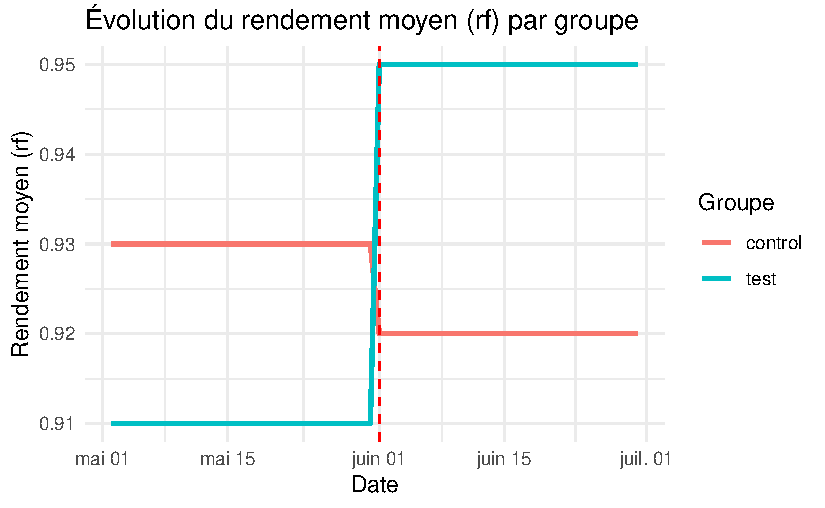
\includegraphics{simulation_modèles_eval_effets_files/figure-pdf/visualisation_data-1.pdf}

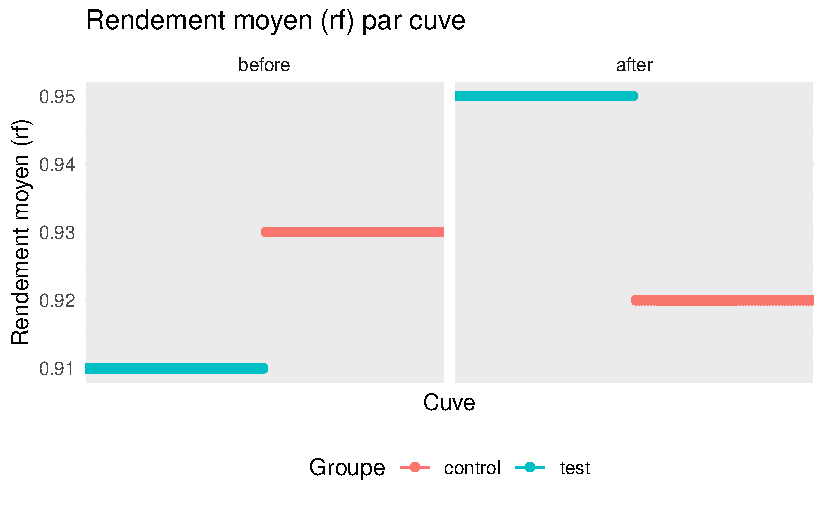
\includegraphics{simulation_modèles_eval_effets_files/figure-pdf/valeurs_rf_cuves-1.pdf}

\begin{longtable*}{ccr}
\caption*{
{\large Moyenne de rf par période et groupe}
} \\ 
\toprule
Période & Groupe & Rendement moyen (rf) \\ 
\midrule\addlinespace[2.5pt]
before & control & $0.930$ \\ 
before & test & $0.910$ \\ 
after & control & $0.920$ \\ 
after & test & $0.950$ \\ 
\bottomrule
\end{longtable*}

\section{Evaluation des modèles sans
variabilité}\label{evaluation-des-moduxe8les-sans-variabilituxe9}

\subsection{Modéle lm avec effets période et groupe sans
interaction}\label{moduxe9le-lm-avec-effets-puxe9riode-et-groupe-sans-interaction}

\begin{quote}
L'effet du test est calculé correctement en sommant les effets de
période après et de groupe test.
\end{quote}

\begin{longtable}[]{@{}ccccc@{}}
\toprule\noalign{}
\endhead
\bottomrule\noalign{}
\endlastfoot
~ & \multicolumn{4}{c@{}}{%
Modèle linéaire sans interaction} \\
Predictors & Estimates & std. Error & Statistic & p \\
(Intercept) & 0.918 & 0.000 & 3595.102 & \textbf{\textless0.001} \\
Période après intervention & 0.015 & 0.000 & 50.901 &
\textbf{\textless0.001} \\
Groupe test & 0.005 & 0.000 & 16.967 & \textbf{\textless0.001} \\
Observations & \multicolumn{4}{l@{}}{%
7200} \\
R\textsuperscript{2} / R\textsuperscript{2} adjusted &
\multicolumn{4}{l@{}}{%
0.286 / 0.286} \\
\end{longtable}

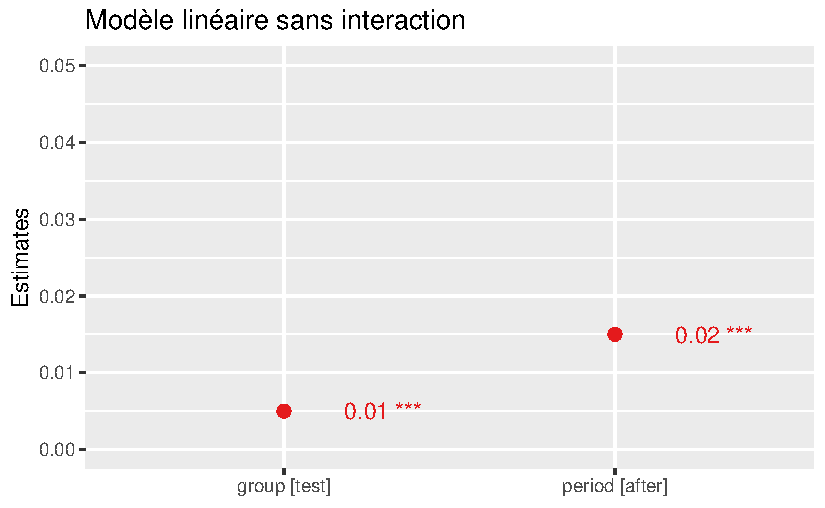
\includegraphics{simulation_modèles_eval_effets_files/figure-pdf/modele_lm_periode_groupe-1.pdf}

\subsection{Modèle lm avec une interaction période et groupe seulement
sans effets
fixes}\label{moduxe8le-lm-avec-une-interaction-puxe9riode-et-groupe-seulement-sans-effets-fixes}

\begin{longtable}[]{@{}ccccc@{}}
\toprule\noalign{}
\endhead
\bottomrule\noalign{}
\endlastfoot
~ & \multicolumn{4}{c@{}}{%
Modèle linéaire avec interaction seulement} \\
Predictors & Estimates & std. Error & Statistic & p \\
(Intercept) & 0.950 & 0.000 & 1516961469183085.000 &
\textbf{\textless0.001} \\
periodbefore:groupcontrol & -0.020 & 0.000 & -22582184034904.504 &
\textbf{\textless0.001} \\
periodafter:groupcontrol & -0.030 & 0.000 & -33873276052357.125 &
\textbf{\textless0.001} \\
periodbefore:grouptest & -0.040 & 0.000 & -45164368069809.078 &
\textbf{\textless0.001} \\
Observations & \multicolumn{4}{l@{}}{%
7200} \\
R\textsuperscript{2} / R\textsuperscript{2} adjusted &
\multicolumn{4}{l@{}}{%
1.000 / 1.000} \\
\end{longtable}

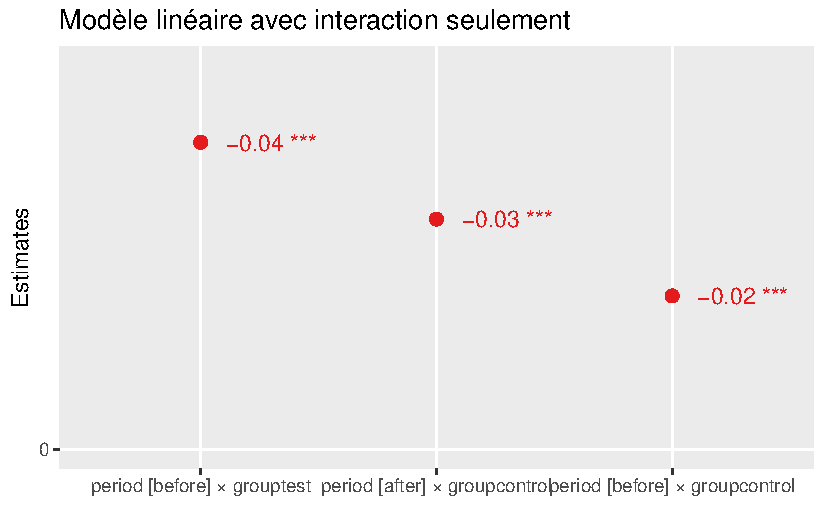
\includegraphics{simulation_modèles_eval_effets_files/figure-pdf/modele_lm_periode_groupe_interaction_seulement-1.pdf}

\subsection{Modéle lm avec effets periode et groupe avec
interaction}\label{moduxe9le-lm-avec-effets-periode-et-groupe-avec-interaction}

\begin{quote}
L'interaction groupe test {[}0, 1{]} x {[}0, 1{]} donne un effet de
+0.05 sur les cuves test après la date d'intervention.

L'effet \emph{Periode Après} donne l'effet du temps indépendamment du
test (Période après x groupe test) et du groupe (effet test) c'est à
dire la baisse pendant la date de l'intervention du groupe de contrôle
(-0.01)

L'effet \emph{Groupe test} donne l'effet du groupe indépendamment du
test (Période après x groupe test) et de l'effet du temps, c'est à dire
l'écart test/ groupe avant (-0.02)
\end{quote}

\begin{longtable}[]{@{}ccccc@{}}
\toprule\noalign{}
\endhead
\bottomrule\noalign{}
\endlastfoot
~ & \multicolumn{4}{c@{}}{%
Modèle linéaire avec interaction} \\
Predictors & Estimates & std. Error & Statistic & p \\
(Intercept) & 0.930 & 0.000 & 1504625977148342.750 &
\textbf{\textless0.001} \\
Période après intervention & -0.010 & 0.000 & -11440120769796.969 &
\textbf{\textless0.001} \\
Groupe test & -0.020 & 0.000 & -22880241539589.723 &
\textbf{\textless0.001} \\
Interaction période: groupe test & 0.050 & 0.000 & 40446934869578.500 &
\textbf{\textless0.001} \\
Observations & \multicolumn{4}{l@{}}{%
7200} \\
R\textsuperscript{2} / R\textsuperscript{2} adjusted &
\multicolumn{4}{l@{}}{%
1.000 / 1.000} \\
\end{longtable}

\section{Evaluation des modèles avec
variabilité}\label{evaluation-des-moduxe8les-avec-variabilituxe9}

\subsection{Visualisation des données avec
variabilité}\label{visualisation-des-donnuxe9es-avec-variabilituxe9}

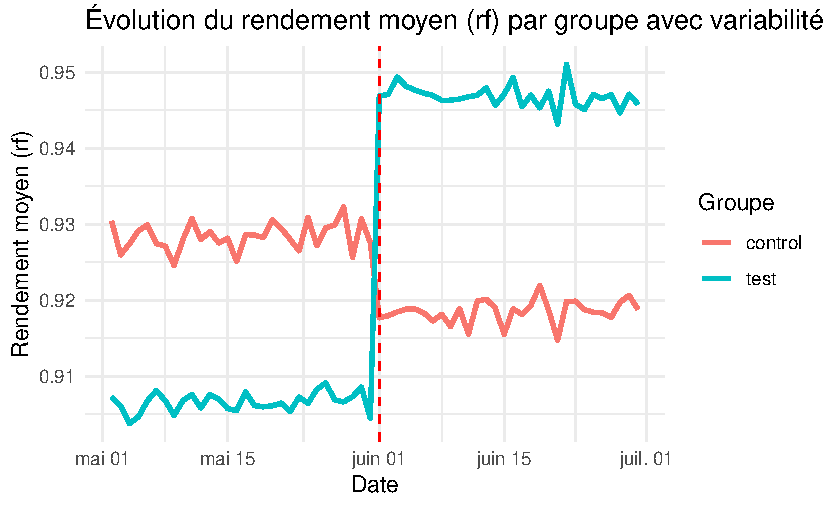
\includegraphics{simulation_modèles_eval_effets_files/figure-pdf/visualisation_data_with_variability-1.pdf}

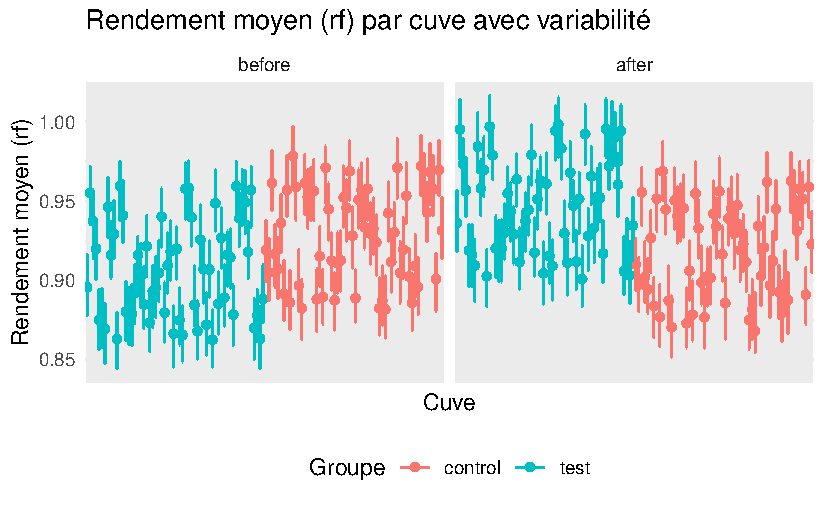
\includegraphics{simulation_modèles_eval_effets_files/figure-pdf/valeurs_rf_cuves_with_variability-1.pdf}

\begin{longtable*}{ccr}
\caption*{
{\large Moyenne de rf par période et groupe avec variabilité}
} \\ 
\toprule
Période & Groupe & Rendement moyen (rf) \\ 
\midrule\addlinespace[2.5pt]
before & control & $0.928$ \\ 
before & test & $0.907$ \\ 
after & control & $0.918$ \\ 
after & test & $0.947$ \\ 
\bottomrule
\end{longtable*}

\subsection{Modéle lmer avec effets période et groupe avec
interaction}\label{moduxe9le-lmer-avec-effets-puxe9riode-et-groupe-avec-interaction}

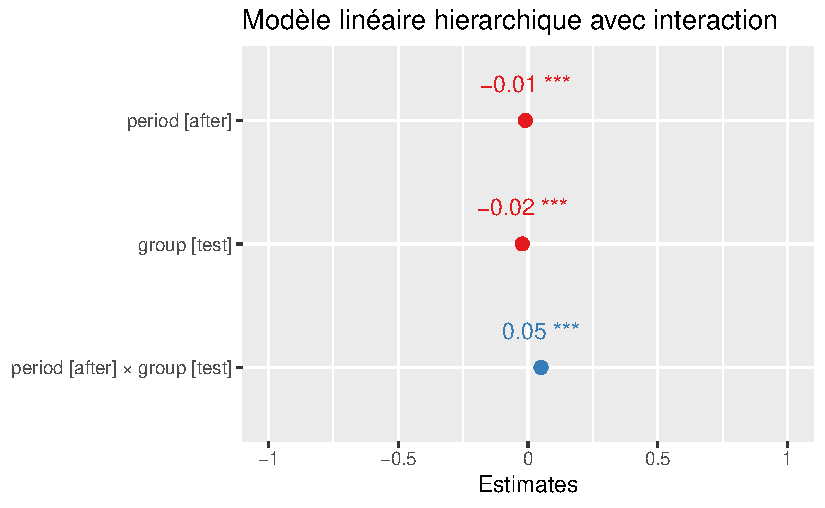
\includegraphics{simulation_modèles_eval_effets_files/figure-pdf/modele_lmer_periode_groupe_with_interaction-1.pdf}

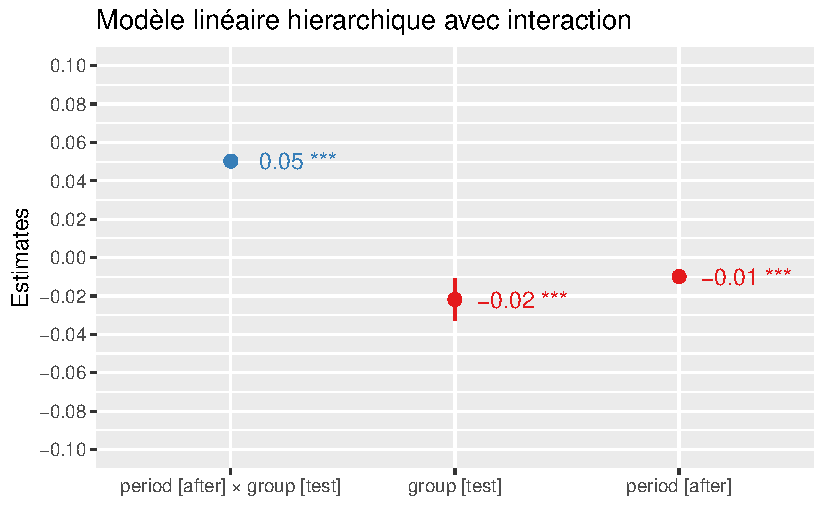
\includegraphics{simulation_modèles_eval_effets_files/figure-pdf/modele_lmer_periode_groupe_with_interaction-2.pdf}

\subsection{Modèle lm avec effets période et groupe avec interaction
pour
référence}\label{moduxe8le-lm-avec-effets-puxe9riode-et-groupe-avec-interaction-pour-ruxe9fuxe9rence}

\begin{longtable}[]{@{}cccccc@{}}
\toprule\noalign{}
\endhead
\bottomrule\noalign{}
\endlastfoot
~ & \multicolumn{5}{c@{}}{%
Modèle linéaire avec interaction pour référence} \\
Predictors & Estimates & std. Error & CI & Statistic & p \\
(Intercept) & 0.928 & 0.001 & -Inf~--~Inf & 1230.901 &
\textbf{\textless0.001} \\
Période après intervention & -0.010 & 0.001 & -Inf~--~Inf & -9.301 &
\textbf{\textless0.001} \\
Groupe test & -0.022 & 0.001 & -Inf~--~Inf & -20.488 &
\textbf{\textless0.001} \\
Interaction période: groupe test & 0.050 & 0.002 & -Inf~--~Inf & 33.280
& \textbf{\textless0.001} \\
Observations & \multicolumn{5}{l@{}}{%
7200} \\
R\textsuperscript{2} / R\textsuperscript{2} adjusted &
\multicolumn{5}{l@{}}{%
0.175 / 0.175} \\
\end{longtable}

\section{Fonction pour extraire le terme
d'interaction}\label{fonction-pour-extraire-le-terme-dinteraction}



\end{document}
